% Source: AESP_466_ClassWork/Supplements/Notes/latex/5.1.3/5.1.3.tex

\documentclass[border=4pt]{standalone}
\usepackage{amsmath,amssymb,amsthm}
\usepackage{graphicx}
\usepackage{tikz}
\usepackage{xcolor}
\usetikzlibrary{arrows.meta,calc,positioning,decorations.markings,patterns,shapes.geometric,angles,quotes,3d}

\definecolor{Garnet}{HTML}{73000A}
\definecolor{USC_Rose}{HTML}{CC2E40}
\definecolor{USC_Blue}{HTML}{466A9F}
\definecolor{USC_Slate}{HTML}{1F414D}
\definecolor{USC_Olive}{HTML}{65780B}
\definecolor{USC_Lime}{HTML}{CED318}
\definecolor{USC_Gold}{HTML}{A49137}
\definecolor{USC_Black90}{HTML}{565556}
\definecolor{USC_Black10}{HTML}{ECECEC}

\newcommand{\vect}[1]{\mathbf{#1}}
\newcommand{\mat}[1]{\mathbf{#1}}
\newcommand{\uvec}[1]{\hat{\mathbf{#1}}}
\newcommand{\transpose}{^{\mkern-1.5mu\mathsf{T}}}
\newcommand{\inv}{^{-1}}
\newcommand{\deriv}[2]{\frac{d #1}{d #2}}
\newcommand{\pderiv}[2]{\frac{\partial #1}{\partial #2}}

\begin{document}
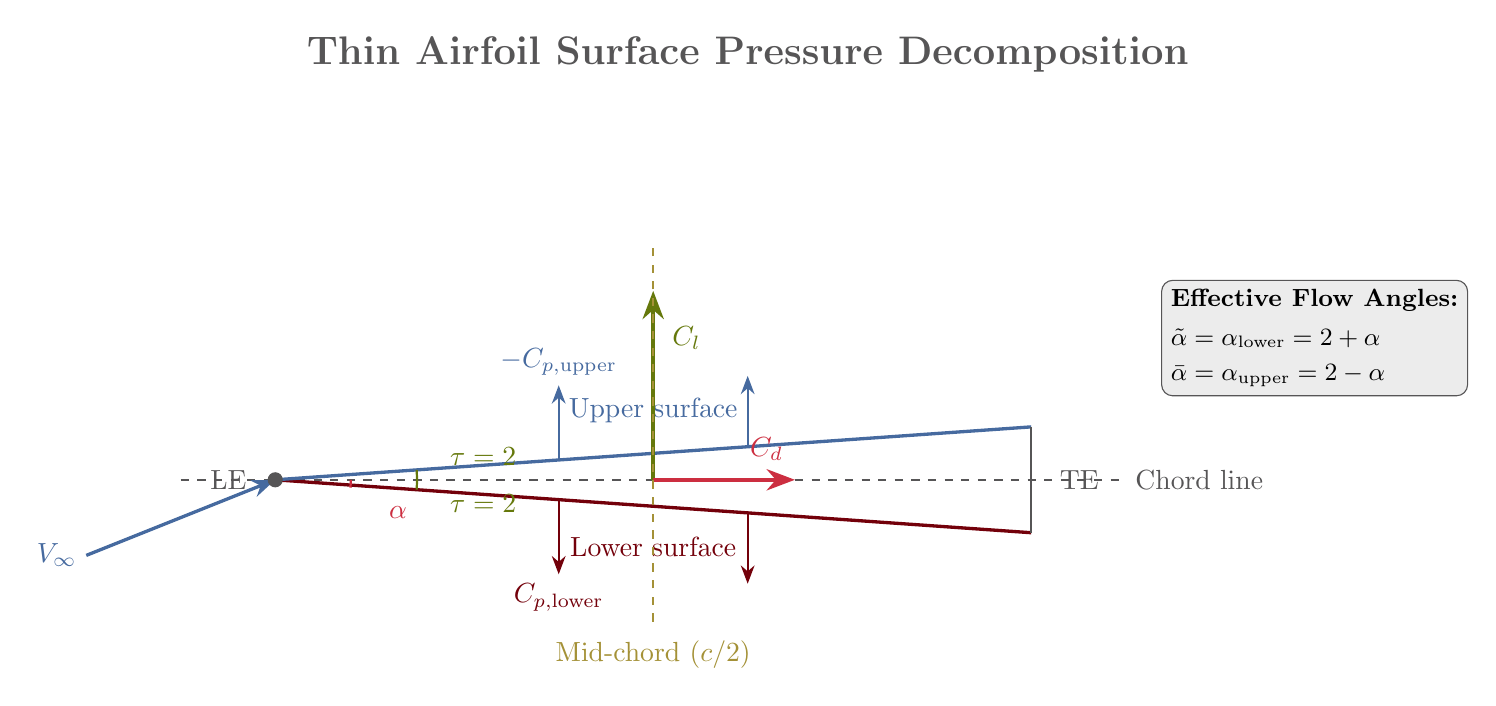
\begin{tikzpicture}[>=Stealth, scale=1.2]
    % Title
    \node[font=\Large\bfseries, USC_Black90] at (5,4.5) {Thin Airfoil Surface Pressure Decomposition};

    % Chord line (horizontal reference)
    \draw[thick, dashed, USC_Black90] (-1,0) -- (9,0);
    \node[USC_Black90, right] at (9,0) {Chord line};

    % Free stream direction (at angle alpha below chord)
    \draw[->, very thick, USC_Blue] (-2,-0.8) -- (0,0);
    \node[USC_Blue, left] at (-2,-0.8) {$V_\infty$};

    % Airfoil surfaces
    % Lower surface (inclined down from leading edge)
    \draw[very thick, Garnet] (0,0) -- (8,-0.56);
    \node[Garnet, below] at (4,-0.5) {Lower surface};

    % Upper surface (inclined up from leading edge)
    \draw[very thick, USC_Blue] (0,0) -- (8,0.56);
    \node[USC_Blue, above] at (4,0.5) {Upper surface};

    % Trailing edge
    \draw[thick, USC_Black90] (8,0.56) -- (8,-0.56);

    % Leading edge point
    \fill[USC_Black90] (0,0) circle (0.08);
    \node[USC_Black90, left] at (-0.2,0) {LE};

    % Trailing edge point
    \node[USC_Black90, right] at (8.2,0) {TE};

    % Wedge angle tau (upper)
    \draw[thick, USC_Olive] (1.5,0) arc[start angle=0, end angle=4, radius=1.5];
    \node[USC_Olive] at (2.2,0.25) {$\tau = 2°$};

    % Wedge angle tau (lower)
    \draw[thick, USC_Olive] (1.5,0) arc[start angle=0, end angle=-4, radius=1.5];
    \node[USC_Olive] at (2.2,-0.25) {$\tau = 2°$};

    % Angle of attack alpha
    \draw[thick, USC_Rose] (0.8,0) arc[start angle=0, end angle=-6, radius=0.8];
    \node[USC_Rose] at (1.3,-0.35) {$\alpha$};

    % Pressure arrows on upper surface
    \draw[->, thick, USC_Blue] (3,0.21) -- (3,1.0);
    \node[USC_Blue, above] at (3,1.0) {$-C_{p,\text{upper}}$};
    \draw[->, thick, USC_Blue] (5,0.35) -- (5,1.1);

    % Pressure arrows on lower surface
    \draw[->, thick, Garnet] (3,-0.21) -- (3,-1.0);
    \node[Garnet, below] at (3,-1.0) {$C_{p,\text{lower}}$};
    \draw[->, thick, Garnet] (5,-0.35) -- (5,-1.1);

    % Effective angles annotation box
    \node[draw=USC_Black90, fill=USC_Black10, rounded corners, align=left, font=\small] at (11,1.5) {
        \textbf{Effective Flow Angles:}\\[0.3em]
        $\tilde{\alpha} = \alpha_{\text{lower}} = 2° + \alpha$\\[0.2em]
        $\bar{\alpha} = \alpha_{\text{upper}} = 2° - \alpha$
    };

    % Lift and drag annotation
    \draw[->, ultra thick, USC_Olive] (4,0) -- (4,2.0);
    \node[USC_Olive, right] at (4.1,1.5) {$C_l$};
    \draw[->, ultra thick, USC_Rose] (4,0) -- (5.5,0);
    \node[USC_Rose, above] at (5.2,0.1) {$C_d$};

    % Mid-chord marker
    \draw[thick, dashed, USC_Gold] (4,-1.5) -- (4,2.5);
    \node[USC_Gold, below] at (4,-1.6) {Mid-chord ($c/2$)};

\end{tikzpicture}
\end{document}
